\documentclass[headheight=4.5cm,
			   margin=2cm,
			   titlewidth=0.6,
			   sansserif,
			   firstcolor=color1,
			   secondcolor=color2,
			   % logo=myLogo.png,
			   % footband=myFootBand.png
               ]{TelecomNancy}
\usepackage{picins}
\usepackage{amssymb}
\usepackage{geometry}
\definecolor{color1}{RGB}{100, 100, 100}
\definecolor{color2}{RGB}{49, 49, 49}


\begin{document}

	\coursetitle{二次函数}
	\courselevel{人教版初中二年级}
	\courseyear{初2017级}
	
	\globalinstructions[二次函数定义相关问题]
	{
		这类问题与二次函数的成立条件相关,\textbf{注意二次项系数不能为0}(即保证$x^2$要存在于函数式中)
	}

	\nextExercise[求满足二次函数条件的参数值]{
		已知函数$y=(kx-1)(x-3)$($k$为常数),根据下列条件求$k$的值:
	}

		\nextQuestion{当$k$为何值时,$y$是$x$的二次函数?}
		\nextQuestion{当$k$为何值时,$y$是$x$的一次函数?}
\bigskip\bigskip\bigskip\bigskip

    \nextExercise{已知函数$y=(m+\frac{3}{2})x^{2m^2+m-1}+mx+1$为关于$x$的二次函数: }

    \nextQuestion{求出$m$的值; }
    \nextQuestion{写出函数关系式. }
    \bigskip\bigskip\bigskip\bigskip\bigskip\bigskip\bigskip\bigskip\bigskip



\globalinstructions[二次函数应用问题]
	{
		这类问题一般需要列出一个二次函数解析式,来帮助解决实际生活中遇到的问题(需要\textbf{注意自变量的取值范围})
	}

	\nextExercise[面积相关问题]{用周长为$20m$的篱笆围成矩形场地: }
    \nextQuestion{场地面积$y$($m^2$)与矩形一边长$x$($m$)之间的关系是什么? (写出自变量的取值范围)}
    \nextQuestion{当边长$x=2$时,求面积$y$的值; }
    \nextQuestion{当面积$y=21$时,求边长$x$的值. }
\bigskip\bigskip\bigskip\bigskip\bigskip\bigskip\bigskip\bigskip\bigskip


	\nextExercise{用19米长的铝合金条制成如图所示的矩形窗框,$CD$长表示窗框的宽,$EF=0.5m$. 若高度$AC$始终大于宽度$CD$,且窗台距天花板$4m$, 求窗框的透光面积$S$(平方米)与窗框的宽$x$(米)之间的函数关系式,并写出自变量的取值范围. (铝合金条的宽度忽略不计)}
\parpic[r]{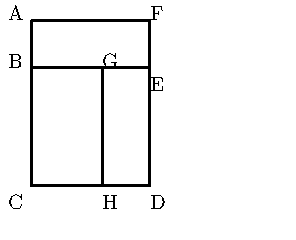
\includegraphics[width=3.5cm]{4.pdf}\label{4}}
    \bigskip\bigskip\bigskip\bigskip\bigskip\bigskip\bigskip\bigskip\bigskip\bigskip\bigskip\bigskip\bigskip


    \nextExercise[需要根据基准判断销量的利润问题]{某商品的进价为每件40元,当售价为每件60元时,每个月可卖出100件;若每件商品的售价每上涨1元,则每个月少卖2件. 设每件商品的售价为$x$元($x$为正整数,且$x\geqslant 60$),每个月的销售利润为$y$元. }

    \nextQuestion{写出$y$与$x$之间的函数关系式,并写出自变量$x$的取值范围; }
    \nextQuestion{在对该商品的总投入不超过2800元的情况下,要使得利润达到2400元,则销售单价应定为多少?}
    \nextQuestion{求销售利润$y$的最大值及对应的$x$的取值. }

\end{document}
